\documentclass[12pt, a4paper]{report}
\usepackage{graphicx} %LaTeX package to import graphics
\usepackage[shortlabels]{enumitem}
\usepackage{geometry}
\usepackage{xcolor}
\geometry{lmargin=30mm}
\usepackage[export]{adjustbox}
\usepackage{titlesec}
\usepackage{float}
\usepackage{listings}

\usepackage{hyperref}

\titleformat{\chapter}{\normalfont\huge}{\thechapter}{20pt}{\huge\bf}
\graphicspath{{images/}} %configuring the graphicx package
\title{Practica 6}
\author{Javier Izquierdo Hernández}
\date{\today}
\begin{document}
	\begin{titlepage}
		\centering
		{
\includegraphics[width=0.3\textwidth]{logo}\par}
		\vspace{1cm}
		{\bfseries\LARGE Universidad Rey Juan Carlos \par}
		\vspace{1cm}
		{\scshape\Large E.T.S. Ingeniería de Telecomunicación \par}
		\vspace{3cm}
		{\scshape\Huge Redes de Ordenadores para Robots y Máquinas Inteligentes \par}
		\vspace{3cm}
		{\itshape\Large Práctica 6\par}
		\vfill
		{\Large Autor: \par}
		{\Large Javier Izquierdo Hernández \par}
		\vfill
		{\Large \today \par}
	\end{titlepage}

\newpage
\renewcommand{\contentsname}{Contenidos}
\tableofcontents
\newpage

\chapter*{Introducción}
En esta práctica debes utilizar mininet-wifi. Ve a la carpeta en la que lo tienes instalado e instala
el módulo para el protocolo B.A.T.M.A.N:
\begin{center}
	\textcolor{blue}{cd mininet-wifi}\\
	\textcolor{blue}{sudo util/install.sh -B}
\end{center}
Descarga tu escenario de red para esta práctica del siguiente enlace:
\begin{center}
	https://mobiquo.gsyc.urjc.es/practicas/ror/p6.html
\end{center}
y descomprime el fichero lab-routing.tgz.
\section*{Capturas de tráfico}
Recuerda que en mininet-wifi puedes capturar tráfico de dos formas diferentes:
\begin{itemize}
	\item\textbf{ Capturar tráfico en la interfaz de un nodo:} Si quieres capturar los paquetes que envía o
	recibe, por ejemplo, sta3:
	\begin{enumerate}
		\item Abre un terminal de sta3 escribiendo en el CLI: \textcolor{blue}{xterm sta3}
		\item Lanza wireshark desde la ventana de sta3 y captura en su interfaz sta3-wlan0 
	\end{enumerate}
	Los paquetes capturados de esta forma no tendrán cabecera 802.11 en su nivel de enlace, sino
	una cabecera Ethernet convencional (802.3) con direcciones de origen y destino convertidas de
	las presentes realmente en 802.11.
	\item \textbf{Capturar todo el tráfico del escenario en la interfaz hwsim0:}
	\begin{enumerate}
		\item En una ventana de la máquina real, escribe: \textcolor{blue}{sudo ifconfig hwsim0 up}
		\item En una ventana de la máquina real, lanza wireshark con sudo.
		\item En wireshark captura en la interfaz hwsim0.
	\end{enumerate}
	En una captura en hwsim0 aparecerán todos los paquetes que envíe cualquier nodo del escenario,
	y los paquetes capturados sí tendrán en su nivel de enlace la cabecera 802.11, con todos sus campos
	de direcciones.
\end{itemize}
\section*{Arrancar y parar batmand en los nodos}
Al arrancar el escenario no estará activado ningún protocolo de routing. Para lanzar el demonio del
protocolo B.A.T.M.A.N. batmand en un nodo, debes ejecutar batmand <nombre\_interfaz>. Así, por
ejemplo, ejecuta en un xterm de sta1):
\begin{center}
	\textcolor{blue}{batmand sta1-wlan0}
\end{center}
También puedes ejecutar desde el CLI: \textcolor{blue}{sta1 batmand sta1-wlan0}\\
Junto con el escenario se incluyen ficheros con órdenes para CLI. La forma de ejecutar las órdenes
de estos ficheros es escribir en el CLI: \textcolor{blue}{source $<$fichero-de-órdenes-CLI$>$}, estando dicho fichero de
órdenes en el mismo directorio desde el que se lanzó mininet-wifi. Así:
\begin{itemize}
	\item \textcolor{blue}{source start-01-04.cli}: Lanza batmand en sta1, sta2, sta3 y sta4.
	\item \textcolor{blue}{source start-05-08.cli}: Lanza batmand en sta5, sta6, sta7 y sta8.
	\item \textcolor{blue}{source start-all.cli}: Lanza batmand en todos los nodos.
\end{itemize}
Para parar batmand en todos los nodos escribe en el xterm de cualquiera de los nodos:
\begin{center}
	\textcolor{blue}{killall batmand}
\end{center}
Para parar batmand en un nodo concreto debes localizar primero el proceso adecuado, identificán-
dolo por el nombre de la interfaz. Por ejemplo, para pararlo en sta1
\begin{center}
	root@raisvm:/home/alumno/p6\# \textcolor{blue}{ps -ef | grep batmand | grep sta1}\\
	root	291668	2144 0 20:33 ?		00:00:01 batmand sta1-wlan0\\
	root@raisvm:/home/alumno/p6\# \textcolor{blue}{kill 291668}
\end{center}
\section*{Ver información del proceso de batmand en ejecución}
Para ver la información que tiene el batmand que se está ejecutando en un nodo ejecuta en un
xterm del nodo:
\begin{center}
	\textcolor{blue}{batmand -c -d 1}
\end{center}
El argumento -c hace que batmand se conecte al demonio que se está ejecutando para obtener la
información del protocolo. El argumento -d 1 permite ver la información de depuración de nivel 1, que
será la que analizaremos en esta práctica:
\begin{figure}[H]
	\centering
	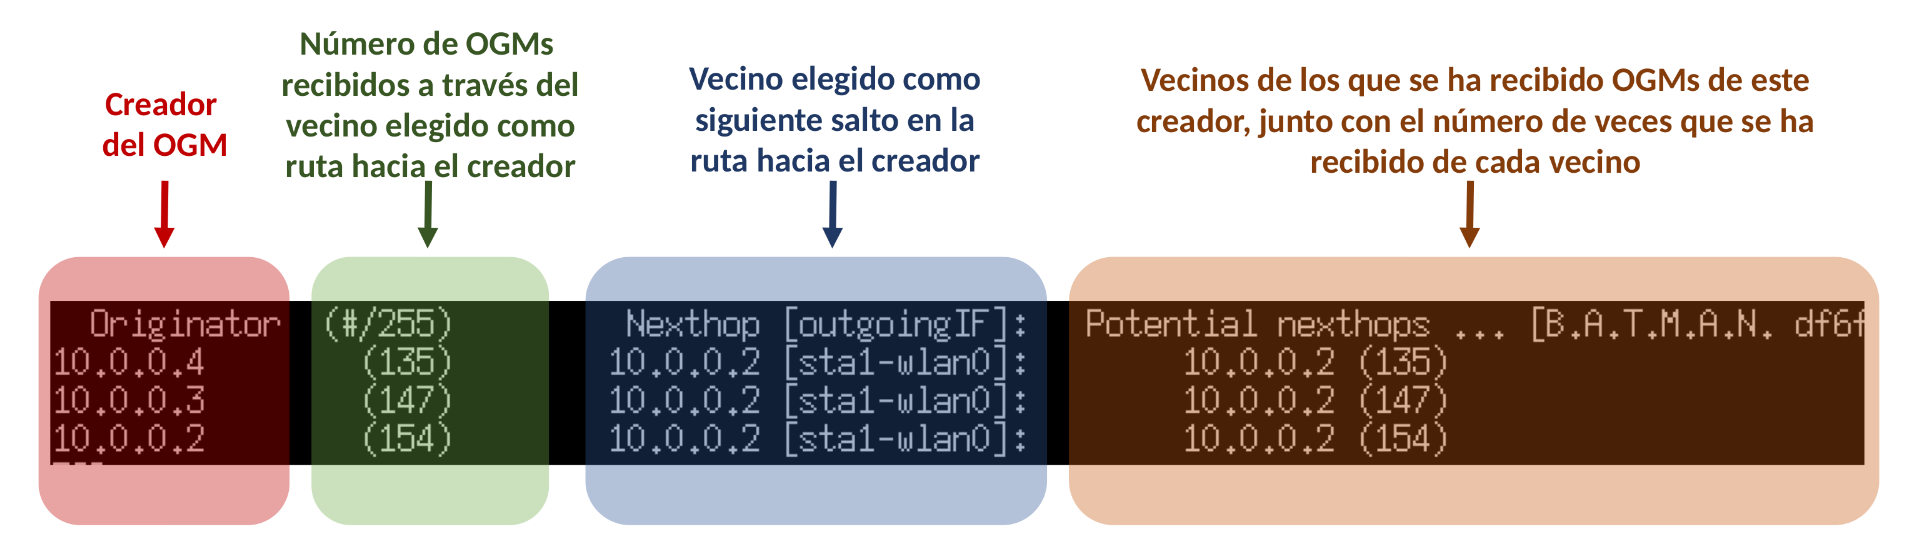
\includegraphics[width=1\textwidth]{enunciado1}
\end{figure}
La información se mostrará continuamente, actualizándose. Para interrumpir la visualización de
información pulsa CTRL-C. Esto NO para la ejecución de batmand en el nodo, sino que simplemente
deja de mostrar la información del mismo.
\section*{Ver la tabla de routing de un nodo}

Normalmente consultamos la tabla de routing de una máquina en Linux con route o con ip route.
Esto muestra la tabla principal del routing de la máquina, pero el kernel de Linux maneja también
otras tablas auxiliares.\\

Por razones de eficiencia, batmand no actúa sobre la tabla principal del nodo, donde sólo se verá una
ruta de vecinos. Así, aunque esté en ejecución batmand y ya haya rutas a través de nodos intermedios,
si se consulta la tabla principal de sta2 desde el CLI con route o ip route sólo se verá su ruta de
vecinos:
\begin{figure}[H]
	\centering
	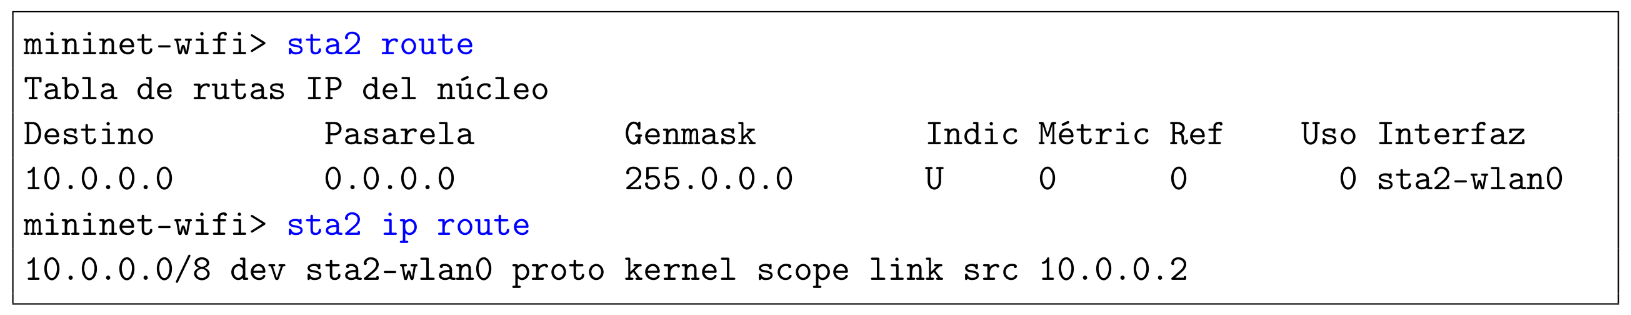
\includegraphics[width=1\textwidth]{enunciado2}
\end{figure}
La tabla de rutas a nodos que usa batmand es la tabla interna número 66, que puede consultarse
con el comando ip route list table 66:
\begin{figure}[H]
	\centering
	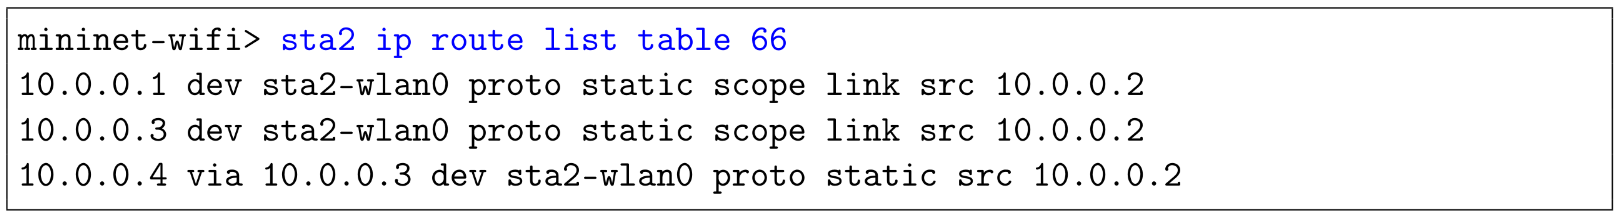
\includegraphics[width=1\textwidth]{enunciado3}
\end{figure}
Así, en la información mostrada, se ve que el nodo sta2 se comunica directamente (dev sta2-wlan0)
con los nodos 10.0.0.1 y 10.0.0.3, pero se comunica con el nodo 10.0.0.4 a través de (via) su vecino
10.0.0.3.
\chapter{Arranque del protocolo B.A.T.M.A.N.}
En el fichero manet-routing.py se encuentra definida una topología de red para Mininet Wifi.
Muévete a la carpeta donde has descomprimido el escenario lab-routing y verás ese fichero.\\

El escenario se arranca de la siguiente forma:
\begin{center}
	sudo ./manet-routing.py
\end{center}
Verás el diagrama que muestra la posición inicial de 8 nodos en configuración de red ad-hoc:
\begin{figure}[H]
	\centering
	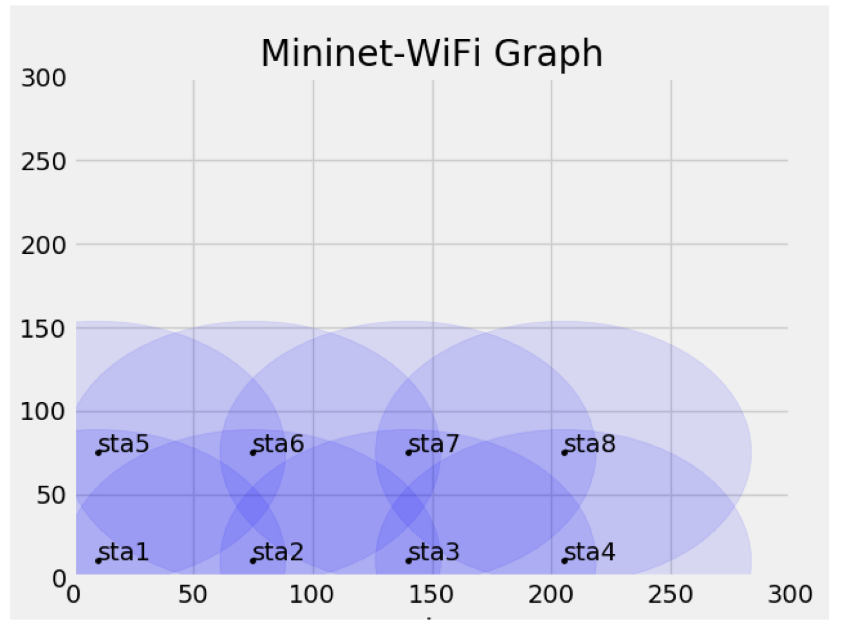
\includegraphics[width=0.6\textwidth]{enunciado4}
\end{figure}
\begin{enumerate}
	\item Comprueba que sólo se pueden comunicar los nodos adyacentes, ejecutando ping entre ellos.
	Si no hay conectividad entre nodos adyacentes, probablemente Mininet Wifi ha arrancado mal:
	ciérralo y vuelve a arrancar el escenario.\\
	
	Para ver de forma reducida la topologia de la red he ejecutado pingallfull como se ve  continuación.
	\begin{figure}[H]
		\centering
		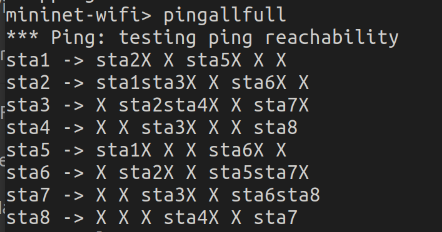
\includegraphics[width=0.5\textwidth]{ej1.1}
	\end{figure}
	\item Activa la interfaz hwsim0 para capturar de forma global en todo el escenario. Ejecuta sudo wireshark
	en la máquina real y empieza a capturar el tráfico de la interfaz hwsim0.\\
	
	Arranca un xterm en sta1, sta2, sta3, sta4.\\
	Arranca batmand en sta1, sta2, sta3, sta4, escribiendo la orden en cada xterm o con ayuda
	del fichero de órdenes CLI, escribiendo en el CLI: \textcolor{blue}{source start-01-04.cli}. Nota: asegúrate de
	que el fichero de órdenes está en la carpeta desde la que has lanzado el CLI o escribe la ruta
	completa a donde se encuentra.\\
	
	Ejecuta en el CLI: \textcolor{blue}{sta1 ping sta4}\\
	
	Tardará en empezar a funcionar. Observa y anota el icmp\_seq de los primeros paquetes de
	ping con respuesta. Cuando el valor del time de los paquetes se estabilice en menos de 30ms,
	interrumpe el ping y la captura.\\
	
	Tarda en empezar funcionar unos 60 ms, y se estabiliza en torno a los 10 ms desde el segundo mensaje (seq=1).\\

	
	En el fichero de captura, filtra los paquetes con filtro ip para quedarte sólo con los paquetes de
	batmand y de icmp.\\
	
	Guarda los paquetes filtrados como captura con nombre de fichero: \textcolor{blue}{batmand-01.pcapng}
	\item Filtra en wireshark los paquetes del B.A.T.M.A.N que tienen IP origen 10.X.0.1 con el filtro:
	bat and ip.src == 10.X.0.1 (sustituyendo la X por el valor que tenga en tu escenario).\\
	Observa que B.A.T.M.A.N. trabaja justo sobre UDP, utilizando el puerto 4305.\\
	El mensaje básico de B.A.T.M.A.N. es el OGM (Originator Message). Observa que 1 solo mensaje
	de BATMAN puede tener varios OGMs concatenados\\
	Observa en los mensajes su IP origen e IP destino. ¿Por qué se envían los OGMs a esa IP destino?\\
	
	Se envían a la Ip destino 10.255.255.255 porque esta engloba a toda la subred, es decir la Ip es la dirección de Broadcast.
	\item Observa los campos principales de los OGMs:
	\begin{itemize}
		\item TTL (en la cabecera de BATMAN, no confundir con el TTL de la cabecera IP): Se le resta
		1 en cada reenvío
		\item Número de secuencia: Se aumenta 1 en cada nuevo OGM que crea un nodo
		\item Originador: Nodo creador del OGM
		\item Reenviado por: Nodo que reenvía el OGM
		\item Calidad de Transmisión (TQ): Valor máximo de 255
	\end{itemize}
	Los mensajes que tienes filtrados son los OGMs reenviados por sta1. Localiza los paquetes en
	que:
	\begin{itemize}
		\item sta1 envía su propio OGM
		\item sta1 reenvía un OGM de sta2
		\item sta1 reenvía un OGM de sta3
		\item sta1 reenvía un OGM de sta4
	\end{itemize}
	Mirando los mensajes con el propio OGM de sta1:
	\begin{itemize}
		\item Observa cómo van aumentando los números de secuencia de los OGMs.\\
		
		El primer mensaje, el del propio OGM de sta1, tiene un número de secuencia de 1, al igual que el que recibe de sta2, ya que tienen enlace directo
		\item ¿Cuál es el periodo de creación de un OGM con nuevo número de secuencia?\\
		
		Es de 1 segundo.
		\item ¿Cuál es el TTL inicial de un OGM?\\
		
		Es 50.
		\item ¿Cuál es la calidad de transmisión de un OGM recién creado?\\
		
		Si el el mensaje es del mismo que lo ha enviado 255, si lo recibe otro es 0 o 1.
	\end{itemize}
	Mirando los mensajes enviados por sta1 reenviando otro OGM: ¿Cómo se explica su valor de
	TTL?\\
	
	El valor del TTl del mensaje proveniente de sta2 es 49 porqué se tiene que enviar una vez (conexión directa), mientras que el de sta3 es 48 porque tiene que ir de sta3 a sta2 y de sta2 a sta1, y por último el de sta4 es de 47 porque tiene que pasar por sta3 y sta2 antes de llegar a sta1.\\

	
	La TQ trata de dar un valor a la calidad de los enlaces entre nodos. Cada vez que un nodo X
	recibe un OGM de un mismo originador O, se fija en el vecino que se lo reenvía y aumenta en uno
	la cuenta de la TQ del enlace entre ambos. Así, el vecino V del que le lleguen más mensajes de
	un mismo OGM (con números de secuencia “cercanos”) será el de mayor calidad de transmisión,
	y V será el siguiente salto en la ruta de X a O.\\
	Cuando un nodo X reenvía un OGM recibido de un vecino V, pondera la TQ que viene en el
	mensaje por la TQ que el nodo X asigna a ese vecino V, y así obtiene la TQ que contendrá el
	OGM reenviado.
	\item Interrumpe batmand en los 4 nodos en que está lanzado, y espera 5 minutos.\\
	No es necesario que vuelvas a capturar tráfico.\\
	Lanza batmand en sta1. Una vez lanzado, ejecuta batmand -c -d 1 para ver la información que
	maneja el nodo sobre los OGMs que va recibiendo, interpretada según la figura de la página 2.
	Como por ahora es el único nodo con el protocolo activado, no verás aún ninguna información.\\
	Lanza ahora batmand en sta2, sta3 y sta4. Ejecuta también en ellos batmand -c -d 1 para ver
	su información.\\
	Observa en los 4 terminales cómo va aumentando la cuenta de los OGMs recibidos en cada nodo.
	Recuerda que esa cuenta representa la TQ del enlace con ese vecino. En los primeros momentos,
	esas TQ son bajas porque aún no han llegado suficientes mensajes. Vuelve a observar en la captura
	anterior como, en efecto, los primeros OGMs que se reenvían tienen una TQ baja hasta que va
	subiendo la cuenta de mensajes recibidos.\\
	
	En la imagen inferior se ven los TQ al pasar un rato.
	\begin{figure}[H]
		\centering
		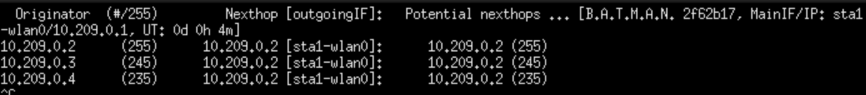
\includegraphics[width=0.8\textwidth]{ej1.5}
	\end{figure}
	\item Consulta la tabla de rutas 66 en cada uno de los 4 nodos, y comprueba su coincidencia con la
	información del protocolo que ves en cada nodo.\\
	
	\textbf{Sta1}: se conecta directamente con sta2, se puede ver que para llegar a sta2 debe ir por sta2, y luego para llegar a sta3 y sta4 debe ir por sta2. En cuanto a los TQ, como sta2 esta al lado el suyo es 255, mientras que cuanto más lejos esta más disminuye.
	\begin{figure}[H]
		\centering
		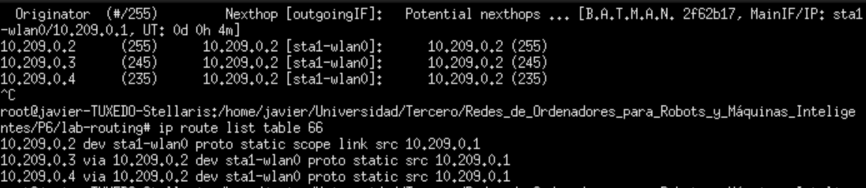
\includegraphics[width=0.8\textwidth]{ej1.6_1}
	\end{figure}
	\textbf{Sta2}: se conecta directamente con sta1 y con sta3, se puede ver con lo explicado anteriormente, y luego para llegar a sta4 debe ir por sta3. En cuanto a los TQ, como sta1 y sta3 estan al lado los suyos serán 255 (o 254), mientras que como sta4 está más lejos es 245.
	\begin{figure}[H]
		\centering
		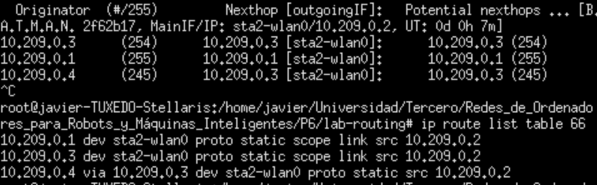
\includegraphics[width=0.8\textwidth]{ej1.6_2}
	\end{figure}
	\textbf{Sta3}: se conecta directamente con sta2 y con sta4, se puede ver con lo explicado anteriormente, y luego para llegar a sta1 debe ir por sta2. En cuanto a los TQ, como sta2 y sta4 estan al lado los suyos serán 255, mientras que como sta1 está más lejos es 242.
	\begin{figure}[H]
		\centering
		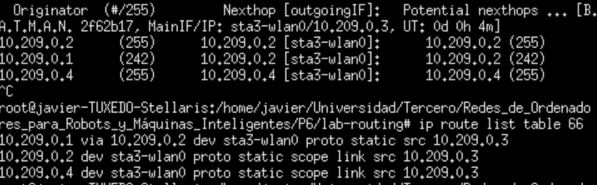
\includegraphics[width=0.8\textwidth]{ej1.6_3}
	\end{figure}
	\textbf{Sta4}: se conecta directamente con sta3, se puede ver que para llegar a sta3 debe ir por sta3, y luego para llegar a sta1 y sta2 debe ir por sta3. En cuanto a los TQ, como sta3 esta al lado el suyo es 253, mientras que cuanto más lejos esta más disminuye.
	\begin{figure}[H]
		\centering
		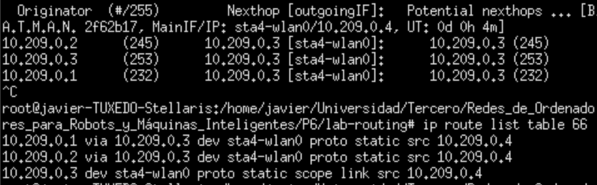
\includegraphics[width=0.8\textwidth]{ej1.6_4}
	\end{figure}
	\item Observa en la captura anterior los mensajes de ICMP. Observa que hay varios echo request y
	varios echo reply por cada número de icmp\_seq: IMPORTANTE – recuerda que estás viendo en
	la captura todos los mensajes enviados y recibidos en todos los nodos.\\
	Busca los mensajes con el primer icmp\_seq del que llegó respuesta al nodo sta1 (es decir, aparece
	un echo reply con ttl=62). Verás que hay 3 echo request y 3 echo reply. ¿Por qué?\\
	
	Porque los mensajes son reenviados por sta2 y sta3, haciendo un total de 3 request (sta1$\rightarrow$sta2, sta2$\rightarrow$sta3, sta3$\rightarrow$sta4) y 3 reply (sta4$\rightarrow$sta3, sta3$\rightarrow$sta2, sta2$\rightarrow$sta1).\\
	
	
	Consulta el TTL de la cabecera IP de cada uno de ellos.\\
	
	El TTl de la cabecera Ip va disminuyendo con cada reenvio: 64$\rightarrow$63$\rightarrow$62.\\
	
	
	Consulta en la cabecera IEEE 802.11 los 4 campos de direcciones (tal y como estudiaste en la
	práctica 4) para confirmar de qué nodo a qué nodo va dirigido cada echo request y cada echo
	reply. Recuerda que los nodos estan trabajando en modo ad-hoc sin access point y las direcciones
	MAC transmitter y source coinciden con el nodo transmisor y las direcciones MAC destination
	y receiver coinciden con el nodo receptor.\\
	Localiza en la captura los mensajes con icmp\_seq menores al primero que obtuvo respuesta en
	el CLI. ¿Por qué no se recibió respuesta para esos icmp\_seq?\\
	
	No hay ??????
\end{enumerate}
\chapter{Arrancar batmand en todos los nodos}
\begin{enumerate}
	\item Arranca un xterm para los nodos sta5 a sta8.\\
	
	Lanza wireshark en sta5 y captura en su interfaz sta5-wlan0, y guarda la captura con nombre
	\textcolor{blue}{batmand-02.pcapng}.\\
	
	Lanza wireshark en sta7 y captura en su interfaz sta7-wlan0, y guarda la captura con nombre
	\textcolor{blue}{batmand-03.pcapng}.\\
	
	Recuerda que ahora en las capturas sólo aparecerán los mensajes enviados o recibidos en ese
	nodo.\\
	
	Arranca batmand en sta5 a sta8. Puedes utilizar el fichero de órdenes de CLI escribiendo en el
	CLI: \textcolor{blue}{source start-05-08.cli}\\
	
	Monitoriza la información del protocolo en los nodos sta5 a sta8 lanzando en cada uno de ellos:
	batmand -c -d 1\\
	
	Ejecuta en CLI: \textcolor{blue}{sta1 ping sta8}\\
	
	Observa en las ventanas de los nodos sta1 a sta4 cómo ellos van conociendo a los 4 nodos nuevos,
	y en la ventanas de los nodos nuevos cómo van conociendo a todos los demás.\\
	
	Anota el tiempo que tarda en comenzar a funcionar el ping.\\
	
	El primer ping tarda en enviarse 100ms y los siguientes a 10ms, por lo tanto podemos deducir que tarda en comenzar a funcionar unos 90 ms.\\
	
	
	Cuando se estabilicen los time, interrumpe el ping y las capturas.
	\item Según la posición de los nodos, las rutas de sta1 hacia sta6, sta7 y sta8 pueden ser a través de
	sta2 o a través de sta5.\\
	
	Observa la información de batmand en sta1. Observa como las rutas hacia sta6, sta7 y sta8
	cambian de vez en cuando entre ser a través de sta2 y ser a través de sta5.\\
	
	En la imagen inferior se ve una captura de la salida de batmand en sta1
	\begin{figure}[H]
		\centering
		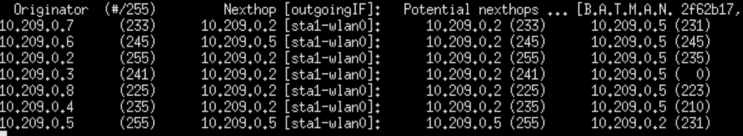
\includegraphics[width=0.8\textwidth]{ej2.2_1}
	\end{figure}
	
	Pon algún otro ejemplo de rutas en otros nodos a los que les ocurra lo mismo.\\
	
	Otro ejemplo de un nodo con las rutas cambiantes es sta4, cuyas rutas para sta6, sta7 y sta5 varían entre sta3 y sta8.\\
	
	Comprueba como se ve la tablas de rutas 66 en cada uno de los nodos.\\
	
	La explicación para sta1 se aplicaría al resto de estaciones cuyas rutas cambian.\\

	\textbf{Sta1}: cuando cambian de sta2 a sta5 las rutas hacia sta6, sta7 y sta8 se ve reflejado en la tabla, donde en vez de aparecer via 10.209.0.2 aparecería 10.109.0.5 o viceversa.
	\begin{figure}[H]
		\centering
		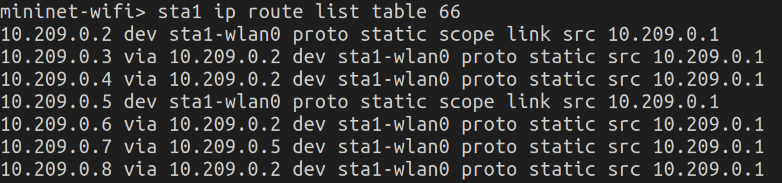
\includegraphics[width=0.8\textwidth]{ej2.2_2}
	\end{figure}
	\textbf{Sta2}
	\begin{figure}[H]
		\centering
		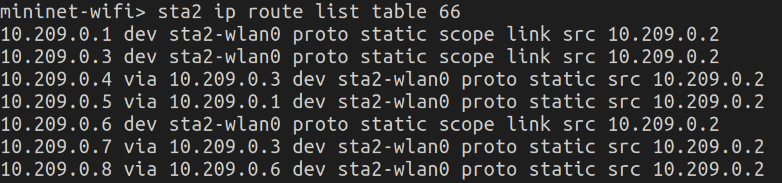
\includegraphics[width=0.8\textwidth]{ej2.2_3}
	\end{figure}
	\textbf{Sta3}
	\begin{figure}[H]
		\centering
		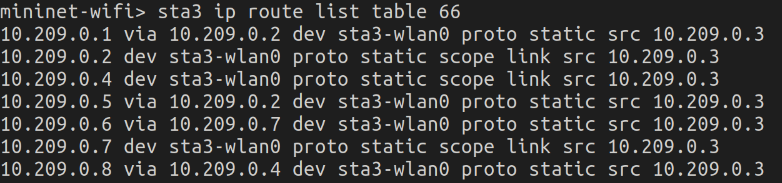
\includegraphics[width=0.8\textwidth]{ej2.2_4}
	\end{figure}
	\textbf{Sta4}
	\begin{figure}[H]
		\centering
		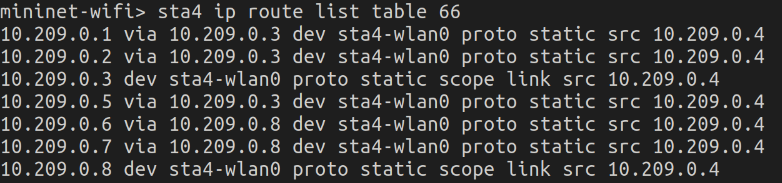
\includegraphics[width=0.8\textwidth]{ej2.2_5}
	\end{figure}
	\textbf{Sta5}
	\begin{figure}[H]
		\centering
		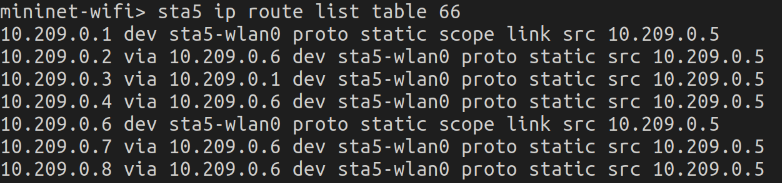
\includegraphics[width=0.8\textwidth]{ej2.2_6}
	\end{figure}
	\textbf{Sta6}
	\begin{figure}[H]
		\centering
		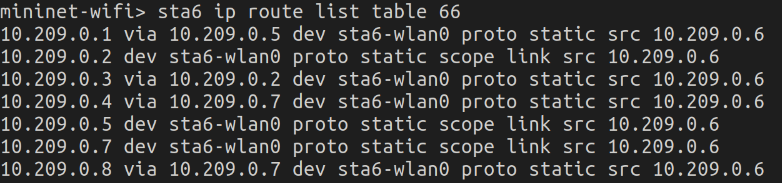
\includegraphics[width=0.8\textwidth]{ej2.2_7}
	\end{figure}
	\textbf{Sta7}
	\begin{figure}[H]
		\centering
		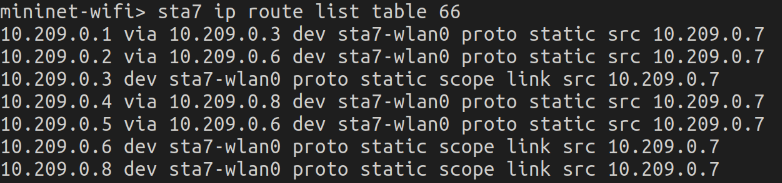
\includegraphics[width=0.8\textwidth]{ej2.2_8}
	\end{figure}
	\textbf{Sta8}
	\begin{figure}[H]
		\centering
		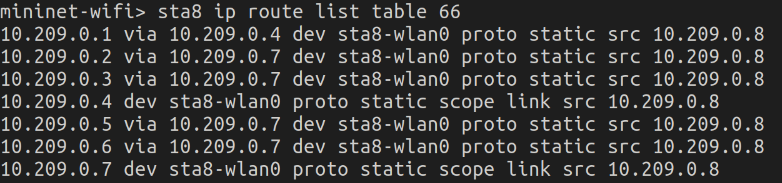
\includegraphics[width=0.8\textwidth]{ej2.2_9}
	\end{figure}
	\item Intenta pensar qué mensajes de ICMP (y con qué direcciones Ethernet) se verán en las 2 capturas
	que has hecho.\\
	
	Abre la captura y localiza esos mensajes. Ten en cuenta que la cabecera de nivel de enlace que
	se ve es de Ethernet normal, 802.3.\\
	
	En la captura sobre sta5 se deberían encontrar mensajes ICMP echo request que vayan desde sta1 a sta5 acompañados de su reenvío de sta5 a sta6.\\
	\begin{figure}[H]
		\centering
		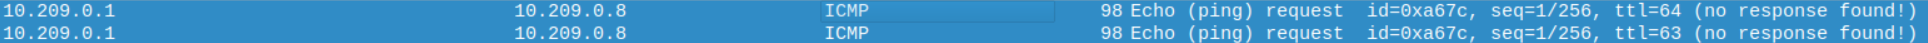
\includegraphics[width=\textwidth]{ej2.3_1}
	\end{figure}
	En la otra captura sobre sta7 se van a encontrar siempre mensajes ICMP echo request que vayan desde sta6 a sta7 y de sta7 a sta8, y se pueden encontrar mensajes de echo reply desde sta8 a sta7 y de sta7 a sta3.
	\begin{figure}[H]
		\centering
		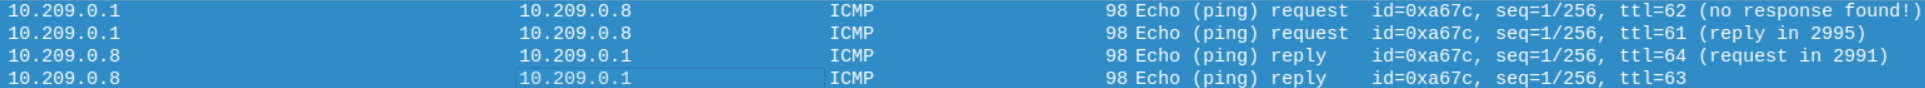
\includegraphics[width=\textwidth]{ej2.3_2}
	\end{figure}	
	\item Localiza en las capturas los OGMs de sta4 y de sta8 reenviados por sta1 y por sta3. Explica
	el valor del TTL del OGM de esos paquetes.\\
	
	En la captura de sta5:\\
	\begin{itemize}
		\item OGM de sta8 reenviado por sta1: TTL = 46\\
		
		Vale siempre 46 y su campo "received from" varía entre sta2 y sta5 ya que para que el mensaje llegue desde sta8 a sta1 debe pasar obligatoriamente por sta2 o sta5 después de haber sido reenviado 2 veces antes
		
		\item OGM de sta4 reenviado por sta1: TTL = 47\\
		
		Vale siempre 47 ya que para que el mensaje llegue desde sta4 a sta1 tiene que ser reenviado por sta2 y sta3.
	\end{itemize}
	
	En la captura de sta7:\\
	\begin{itemize}
		\item OGM de sta8 reenviado por sta3: TTL = 48\\
		
		Vale siempre 48 y su campo "received from" varía entre sta4 y sta7 ya que para que el mensaje llegue desde sta8 a sta3 debe pasar obligatoriamente por sta4 o sta7
		\item OGM de sta8 reenviado por sta3: TTL = 49\\
		
		Vale siempre 49 ya que para que el mensaje llegue desde sta4 a sta3 no hace falta que se reenvie el mensajes.
	\end{itemize}
\end{enumerate}
\chapter{Cambio de posición de nodos}
\begin{enumerate}
	\item Lanza wireshark en sta3 y captura en su interfaz sta3-wlan0, y guarda la captura con nombre
	\textcolor{blue}{batmand-04.pcapng}.\\
	
	Lanza wireshark en sta7 y captura en su interfaz sta7-wlan0, y guarda la captura con nombre
	\textcolor{blue}{batmand-05.pcapng}.\\
	
	Asegúrate de que sigues viendo la información del protocolo en los nodos.\\
	
	Cambia de posición a sta7 y a sta8 con las siguientes órdenes en CLI:
	\begin{center}
		\textcolor{blue}{py sta7.setPosition('10,205,0')}\\
		\textcolor{blue}{py sta8.setPosition('10,270,0')}
	\end{center}
	Tras esto, la posición de los nodos resultará ser:
	\begin{figure}[H]
		\centering
		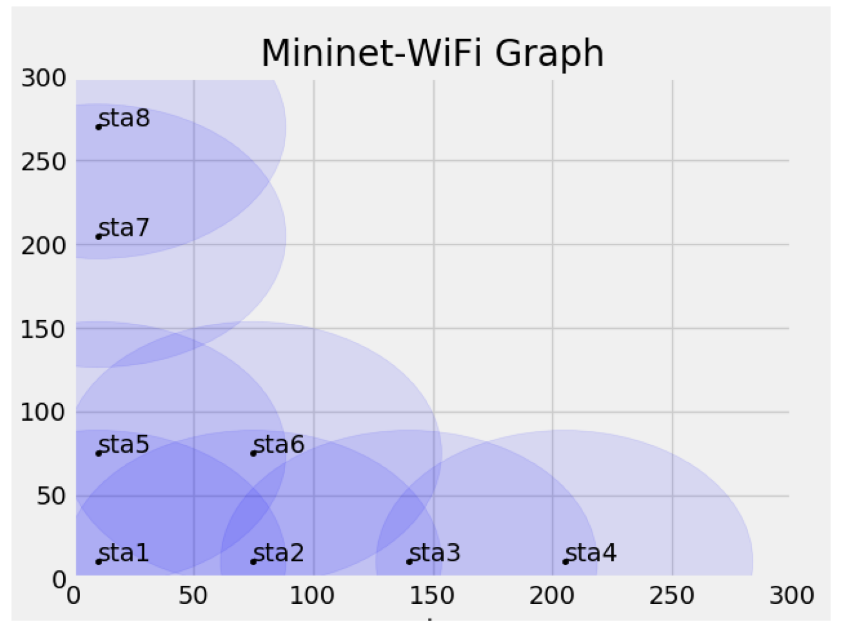
\includegraphics[width=0.6\textwidth]{enunciado5}
	\end{figure}
	Ejecuta en CLI: \textcolor{blue}{sta1 ping sta8}\\
	
	Observa la información del protocolo en sta3 y sta5. Observa la evolución de los valores de TQ
	de los enlaces a los nodos que se han movido.\\
	
	Observa la información del protocolo en sta7 y sta8. Observa la evolución de los valores de TQ
	de los enlaces entre sí y al resto de los nodos.\\
	
	Ejecuta en CLI: \textcolor{blue}{sta7 ping sta8}\\
	
	Interrumpe las capturas.\\
	
	Intenta pensar qué mensajes de B.A.T.M.A.N. y de ICMP vas a ver en cada captura. Comprueba
	que tus suposiciones son ciertas.\\
	
	En la captura realizada sobre sta7 se verá que antes de moverse recibe los mensajes de BATMAN del resto de estaciones, mientras que después de desplazarse solo se intercambiaran mensajes de BATMAN con sta8. Y en cuanto a los mensajes ICMP se enviarán sin problema alguno.
	
	En la captura realizada en sta3 se verá que antes de moverse sta7 y sta8, recibe los mensajes de BATMAN del resto de estaciones, mientras que después de desplazarse estas 2 estaciones desaparecen. En cuanto a los mensajes ICMP no tendrán respuesta y si la tienen será de Host Unreachable.
	\item Lanza wireshark en sta5 y captura en su interfaz sta5-wlan0, y guarda la captura con nombre
	\textcolor{blue}{batmand-06.pcapng}.\\
	
	Lanza wireshark en sta7 y captura en su interfaz sta7-wlan0, y guarda la captura con nombre
	\textcolor{blue}{batmand-07.pcapng}.\\
	
	Asegúrate de que sigues viendo la información del protocolo en los nodos.\\
	
	Cambia de posición a sta4 con la siguiente orden en CLI:
	\begin{center}
		\textcolor{blue}{py sta4.setPosition('10,140,0')}
	\end{center}
	Tras esto, la posición de los nodos resultará ser:
	\begin{figure}[H]
		\centering
		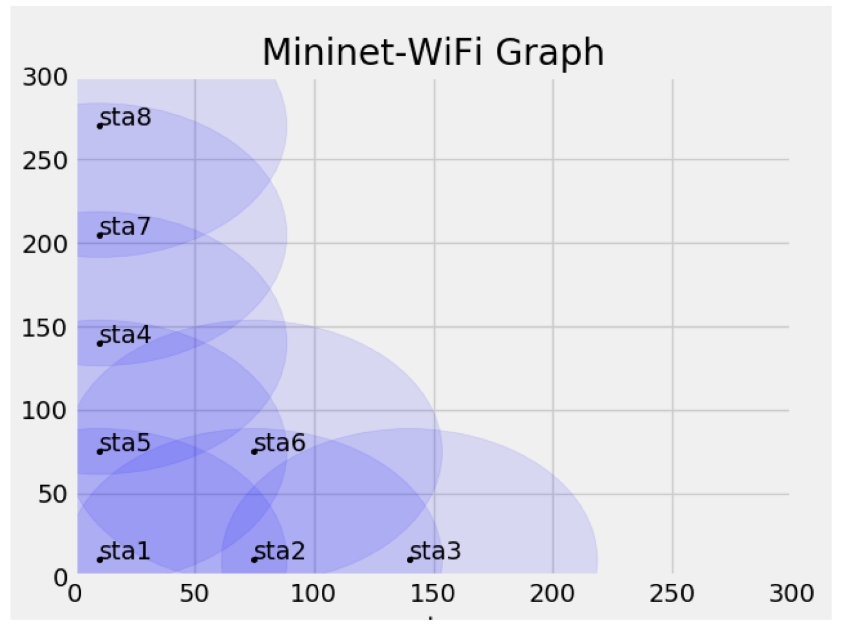
\includegraphics[width=0.6\textwidth]{enunciado6}
	\end{figure}
	Ejecuta en CLI: \textcolor{blue}{sta1 ping sta8}\\
	
	Anota el tiempo que tarda en funcionar el ping. Cuando se estabilice el valor de time interrumpe
	las capturas.\\
	
	Aprox 75 ms.
	\begin{figure}[H]
		\centering
		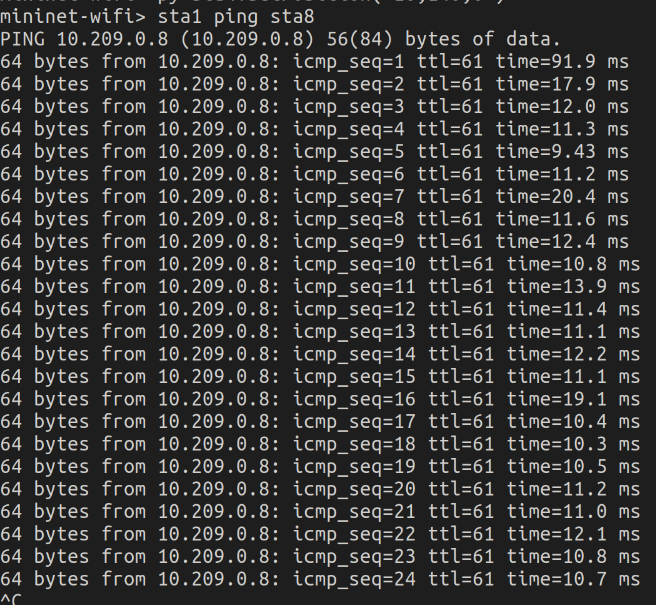
\includegraphics[width=0.8\textwidth]{ej3.2}
	\end{figure}
	
	Observa la información del protocolo en sta4 y sta7. Observa la evolución de los valores de TQ
	de los enlaces.\\
	
	Intenta pensar qué mensajes de B.A.T.M.A.N. y de ICMP vas a ver en cada captura. Comprueba
	que tus suposiciones son ciertas.\\
	
	En la captura realizada en sta7 se ve que al comienzo ocurre lo mismo que se ha explicado en la pregunta anterior después de moverse. Cuando se mueve sta4, sta7 empieza a recibir los mensajes de BATMAN del resto de las estaciones a través de sta4, y por lo tanto recibirá los ping realizados.\\
	
	En la captura realizada en sta5 se verá que al principio solo recibe datagramas de BATMAN de las estaciones 1, 2, 3, 4, 5 y 6. Cuando sta4 se mueve sta5 recibirá los datagramas de sta7 y sta8 a través de sta4. Como todos las estaciones están conectadas entre si los mensajes ICMP funcionarán sin problema alguno.
\end{enumerate}
\end{document}